\documentclass{beamer}
%\usepackage[portuges]{babel}
\usepackage[latin1]{inputenc}
\usepackage[T1]{fontenc}
\usepackage{fancyvrb}
\usepackage{url}
\usepackage{verbatim}
\usepackage{graphics}
%\usepackage{beamerthemecopenhagen}
\usetheme{Malmoe}
%\usepackage{beamerthemeCopenhagen}
\usepackage{graphicx}
\setbeamertemplate{footline}[page number]
\setbeamertemplate{navigation symbols}{}
\usepackage{listings}
\input{jml-listings}
\lstset{language=[JML]Java,basicstyle=\ttfamily,commentstyle=\ttfamily,
        showstringspaces=false,
        keywordstyle=\bfseries,
        keywordstyle={[2]\bfseries\color{violet!80!black}}
       }


\title{Connecting between VDM++ and JML}
\author{Carlos Vilhena}
\institute{Engineering College of Aarhus}
\date{\today}

\begin{document}

\frame{\titlepage}

\section{Agenda}

\frame{
\frametitle{Agenda}
\begin{itemize}
\item Introduction
\item Correlation between VDM++ and JML
\item Requirements Specification
\item Connection's Architecture
\item Future Work
\item Questions
\end{itemize}
}

\section{Introduction}
\subsection{Purpose}
\frame{
\frametitle{Purpose of this project}
Map VDM++ to JML
\newline
\newline
\pause
Map JML to VDM++
\newline
\newline
\pause
Assemble in Eclipse
}
\subsection{Motivation}
\frame{
\frametitle{Motivation}
\begin{itemize}
\item Teaching perspective: VDM++ as front-end to Design by Contract programming
\newline
\newline
\pause
\item Tool Support
\newline
\newline
\pause
\item Java code generator + JML assertions generator
\end{itemize}
}
\subsection{General Overview}
\frame{
\frametitle{VDM++}
\ldots
}
\frame{
\frametitle{JML}
Behavioural Interface Specification Language
\newline
\newline
\pause
Used to specify behaviour of Java modules
\newline
\newline
\pause
Design by Contract approach
\newline
\newline
\pause
Assertions as Java annotations
\newline
\newline
\pause
Multiple usage: class, abstract class and interface
}

\section{Correlation between VDM++ and JML}
\subsection{Basic Types}
\frame{
\frametitle{}
\begin{itemize}
\item \textit{Character} $\approx$ \textit{JMLChar}
\pause
\newline
\item \textit{Quote} $\approx$ \textit{JMLEnumeration}
\pause
\newline
\item \textit{Boolean} $\approx$ \textit{Java boolean}
\pause
\newline
\item . . .
\end{itemize}
}
\subsection{Compound Types}
\frame{
\frametitle{}
\begin{itemize}
\item \textit{Set} $\approx$ \textit{JMLValueSet}
\pause
\newline
\item \textit{Map} $\approx$ \textit{JMLValueToValueMap}
\pause
\newline
\item \textit{Seq} $\approx$ \textit{JMLValueSeq}
\pause
\newline
\item . . .
\end{itemize}
}
\frame{
\frametitle{Compound Types (cont.)}
VDM++ Records are different
\newline
\newline
\pause
Composed with a number of types
\newline
\newline
\pause
Correspond to Class in Java
}

\subsection{Language semantics}
\frame{
\frametitle{Pre-Conditions}
\begin{itemize}
\item VDM++ pre-condition: \textit{pre} Expression
\newline
\newline
\pause
\item JML requires clause: \textit{requires} Expression
\newline
\newline
\pause
\item Both respect same principles
\end{itemize}
}
\frame{
\frametitle{Post-Conditions}
\begin{itemize}
\item VDM++ post-condition: \textit{post} Expression
\newline
\newline
\pause
\item JML ensures clause: \textit{ensures} Expression
\newline
\newline
\pause
\item Both respect same principles
\end{itemize}
}
\frame{
\frametitle{Exception Conditions}
\begin{itemize}
\item VDM++ \textit{errs}: \textit{errs} COND: c -> r
\newline
\newline
\pause
\item JML ensures clause: \textit{signals} (E e) P;
\newline
\newline
\pause
\item Both respect same principles
\end{itemize}
}
\frame{
\frametitle{Invariants}
VDM++ allows:
\begin{itemize}
\item Type invariants
\item Instance Invariants
\end{itemize}
\pause
JML allows:
\begin{itemize}
\item Static invariants
\item Instance Invariants
\end{itemize}
\pause
Question: How to map VDM++ Type invariants?
}
\frame{
\frametitle{Type Invariants}
Record: type invariant $\equiv$ instance invariant
\newline
\newline
\pause
Otherwise, there are two possibilities:
\begin{itemize}
\item Instantiate the invariant for each variable using the type
\newline
\pause
\item "Extend" pre-defined JML types with invariant
\end{itemize}
\pause
Solution?
}


\section{Requirements Specification}

\subsection{Overview}
\frame{
\frametitle{Intention}
\begin{figure}[!htb]
\begin{center}
\resizebox{.60\textwidth}{!}{\includegraphics{figures/main.ps}}
\end{center}
\end{figure}
}
\subsection{g: VDM++ $\rightarrow$ JML}
\frame{
\frametitle{Parsing and AST generation}
\begin{figure}[!htb]
\begin{center}
\resizebox{.99\textwidth}{!}{\includegraphics{figures/vdmParser.ps}}
\end{center}
\end{figure}
}
\frame{
\frametitle{Converting ASTs and generating JML code}
\begin{figure}[!htb]
\begin{center}
\resizebox{.99\textwidth}{!}{\includegraphics{figures/vdmConvertAsts.ps}}
\end{center}
\end{figure}
}
\subsection{f: JML $\rightarrow$ VDM++}
\frame{
\frametitle{Parsing JML files and AST generation}
\begin{figure}[!htb]
\begin{center}
\resizebox{.86\textwidth}{!}{\includegraphics{figures/diagramaChecker.ps}}
\end{center}
\end{figure}
}
\frame{
\frametitle{AST conversion}
\begin{figure}[!htb]
\begin{center}
\resizebox{.99\textwidth}{!}{\includegraphics{figures/diagramaConvertASTs.ps}}
\end{center}
\end{figure}
}
\frame{
\frametitle{VDM++ code generation}
\begin{figure}[!htb]
\begin{center}
\resizebox{.99\textwidth}{!}{\includegraphics{figures/diagramaJMLVDM.ps}}
\end{center}
\end{figure}
}
\subsection{Tool support to use}
\frame{
\frametitle{Tool support}
VDM++/Overture tool support:
\newline
\pause
\begin{itemize}
\item Overture parser
\pause
\item Overture AST generator
\pause
\item VDMTools Java Code Generator
\pause
\end{itemize}
JML tool support:
\newline
\pause
\begin{itemize}
\item JML Checker
\end{itemize}
}

\subsection{Tool support to develop}
\frame{
\frametitle{Tool support}
\begin{itemize}
\item JML abstract syntax tree
\pause
\item JmlAst to JmlAstVdm mapper
\pause
\item JmlAstVdm to Vdm++Ast mapper
\pause
\item Vdm++Ast to JmlAstVdm mapper
\pause
\item pretty printer(s)...
\end{itemize}
}

\section{Connection's Architecture}

\subsection{Purpose}
\frame{
\frametitle{}
\begin{figure}[!htb]
\begin{center}
\resizebox{.90\textwidth}{!}{\includegraphics{figures/image1.ps}}
\end{center}
\end{figure}
\pause
How To?
}

\subsection{Mapper}
\frame{
\frametitle{}
\begin{figure}[!htb]
\begin{center}
\resizebox{.99\textwidth}{!}{\includegraphics{figures/image2.ps}}
\end{center}
\end{figure}
}
\subsection{Core}
\frame{
\frametitle{}
\begin{figure}[!htb]
\begin{center}
\resizebox{.99\textwidth}{!}{\includegraphics{figures/image3.ps}}
\end{center}
\end{figure}
}
\subsection{Control Panel}
\frame{
\frametitle{}
\begin{itemize}
\item Error/Warning Messages
\pause
\newline
\item Decisions
\pause
\newline
\item Limitations log
\end{itemize}
}

\section{Future}

\frame{
\frametitle{Future work}
\begin{itemize}
\item Generate AST from JML input files in JML checker
\newline
\pause
\item Continuing building tool support and assemble in eclipse plugin
\newline
\pause
\item GUI
\newline
\pause
\item Continuing writing thesis
\end{itemize}
}

\section{Questions}

\frame{
\frametitle{}
\Huge Questions?
}

\end{document}